\subsection{SnakeManager}
\label{section:SnakeManager}

The SnakeManager has the responsibility for handling all game logic having to do with the snake. Its primary areas of concern are: Initializing and updating an array representing the snake array, adding a new body part to the snake when it hits a piece of food, and detecting whether or not the snake collides with itself.

Figure \ref{SnakeManagerClassDiagram} shows a class diagram of the SnakeManager.

\begin{figure}[H]
	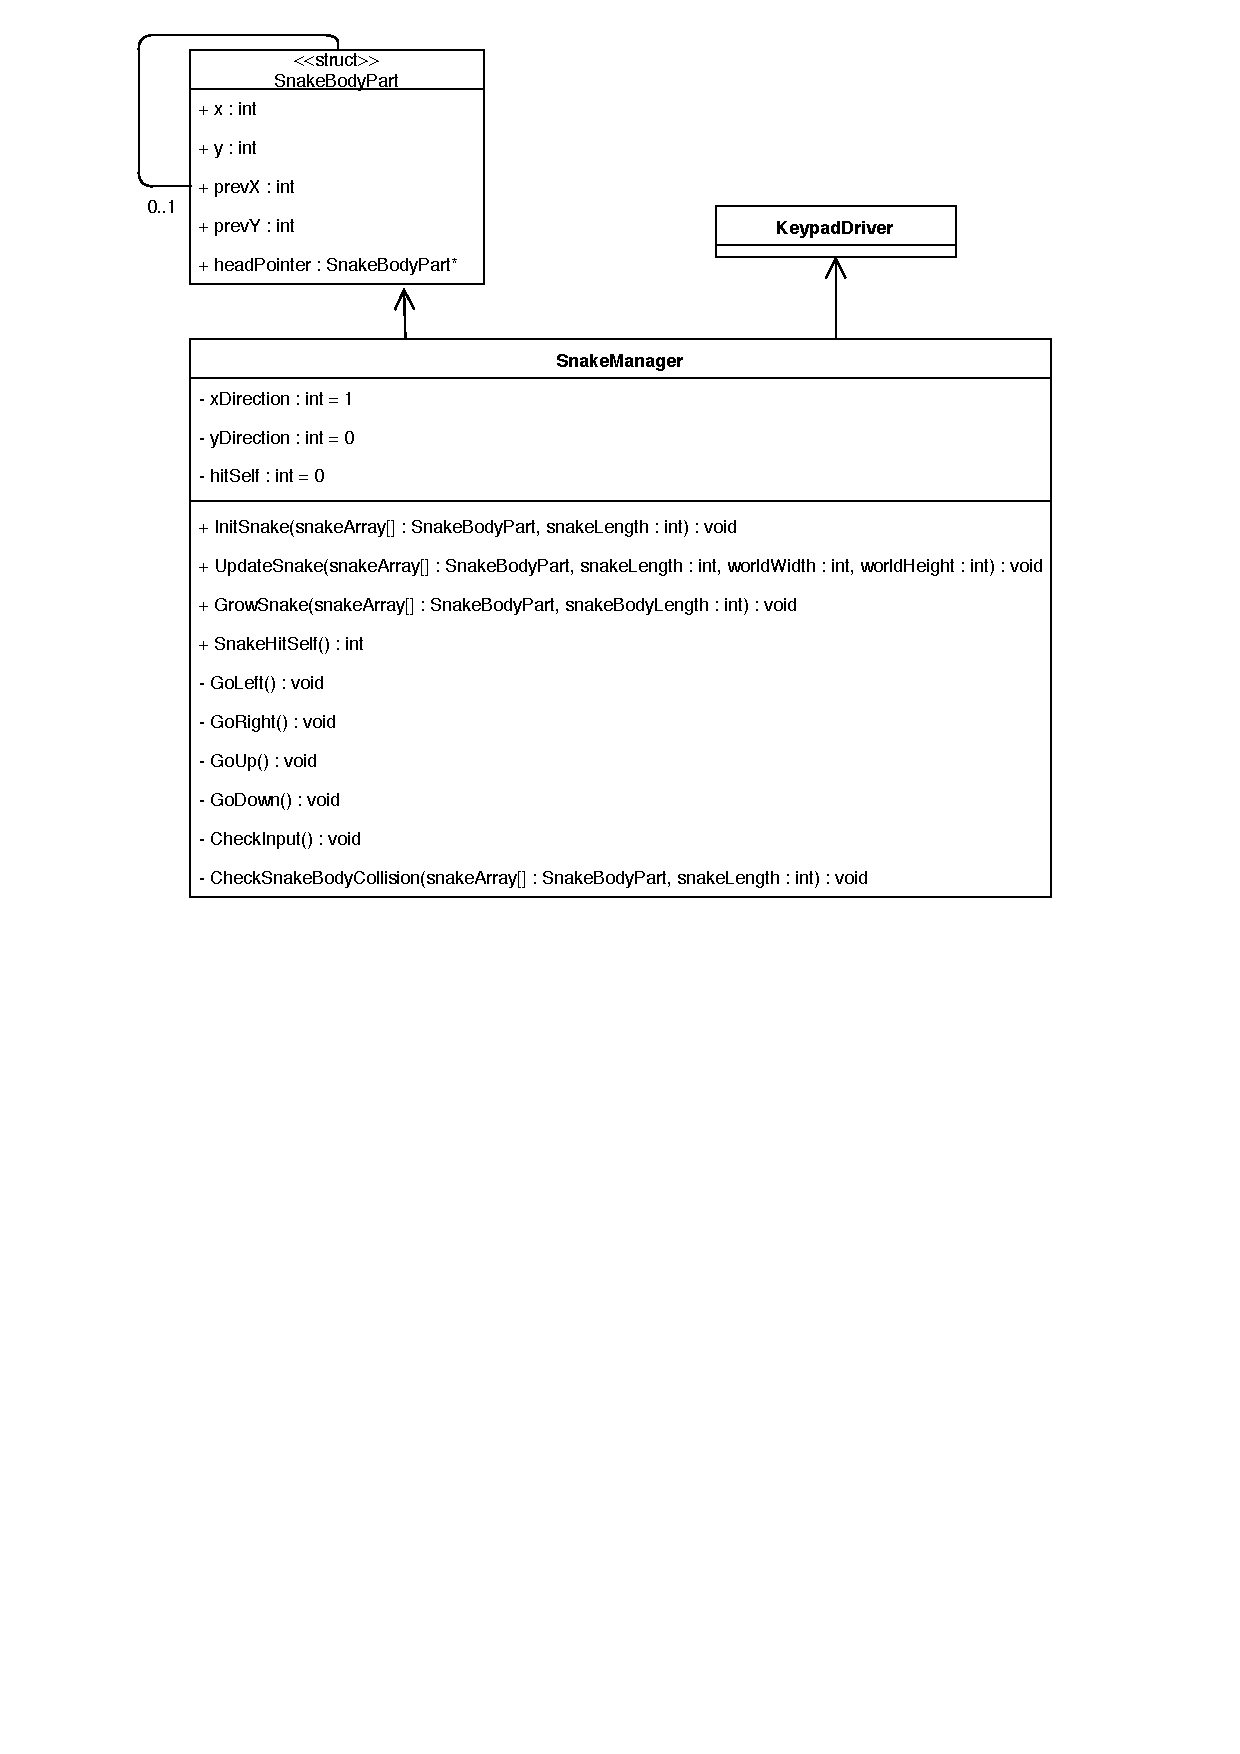
\includegraphics[scale=0.75]{SnakeManagerClassDiagram}
	\centering
	\caption{Class diagram for SnakeManager}
	\label{SnakeManagerClassDiagram}
\end{figure} 

As can be seen in figure \ref{SnakeManagerClassDiagram}, The SnakeManager makes use of the KeypadDriver. This driver is described in section \ref{section:MatrixKeyboard} - \nameref{section:MatrixKeyboard}.

Also, the SnakeManager makes use of a struct by the name of SnakeBodyPart. This struct represents a single part of the snake's body. It is by these body parts that the snake grows - one by one. 

Table \ref{table:SnakeBodyPartAttributeDescriptions} contains descriptions of the attributes of the SnakeBodyPart struct.

\begin{table}[H]
	\centering
	\begin{tabular}{|l|l|}
		\hline
		Attribute & Description \\ \hline
		x & The X position of the body part in world space. \\ \hline
		y & The Y position of the body part in world space. \\ \hline
		prevX & \begin{tabular}[c]{@{}l@{}}The X position of the body part in the\\ previous frame of the game loop.\end{tabular} \\ \hline
		prevY & \begin{tabular}[c]{@{}l@{}}The Y position of the body part in the previous\\ frame of the game loop.\end{tabular} \\ \hline
		headPointer & \begin{tabular}[c]{@{}l@{}}A pointer to the SnakeBodyPart which this\\ SnakeBodyPart is chained to.\end{tabular} \\ \hline
	\end{tabular}
	\caption{Descriptions of the attributes for the SnakeBodyPart struct, used by the SnakeManager}
	\label{table:SnakeBodyPartAttributeDescriptions}
\end{table} 

The way that the snake is represented and managed through the game is by an array of the aforementioned SnakeBodyPart structs. Figure \ref{SnakeBodyPartManagement} illustrates this.

\begin{figure}[H]
	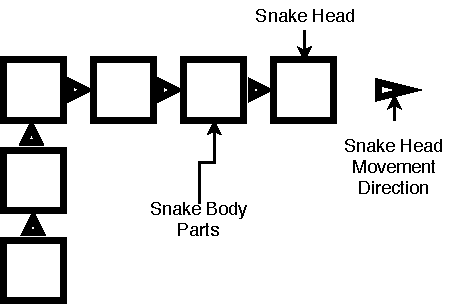
\includegraphics[scale=1.0]{SnakeBodyPartManagement}
	\centering
	\caption{Illustration of the snake being made up of a chain of SnakeBodyParts}
	\label{SnakeBodyPartManagement}
\end{figure} 

Essentially, the snake is a linked list \cite{LinkedLists} of SnakeBodyParts. Each SnakeBodyPart, as mentioned in table \ref{table:SnakeBodyPartAttributeDescriptions}, has a pointer to a SnakeBodyPart that comes next in the chain. it's a recursive struct.

Every time the game advances a single frame, the head of the snake moves a certain amount of world units in a direction determined by the user. Afterwards, each chained SnakeBodyPart advances themselves to the previous position of its chained SnakeBodyPart. This makes all parts of the snake move as a coherent whole. This update process is illustrated in figure \ref{SnakeBodyPartUpdateProcess}.

\begin{figure}[H]
	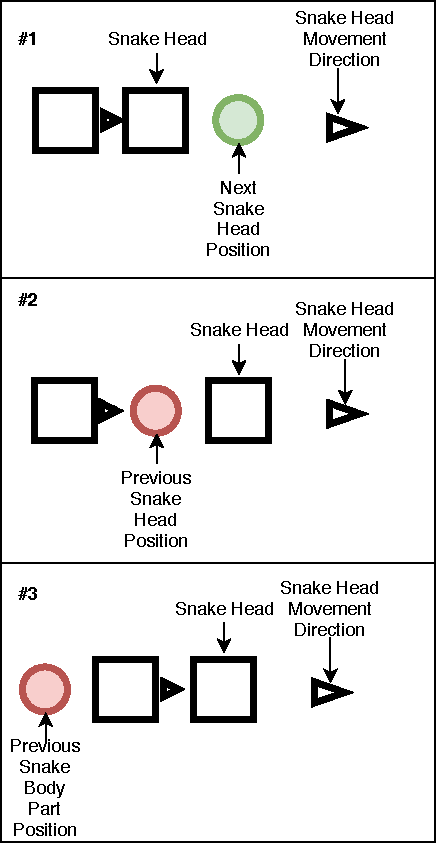
\includegraphics[scale=0.75]{BodyPartsUpdatingIllustration}
	\centering
	\caption{Illustration of the SnakeBodyPart update process}
	\label{SnakeBodyPartUpdateProcess}
\end{figure} 

Table \ref{table:SnakeManagerAttributeDescriptions} contains descriptions for the attributes of SnakeManager.

\begin{table}[H]
	\centering
	\begin{tabular}{|l|l|}
		\hline
		Attribute & Description \\ \hline
		xDirection & \begin{tabular}[c]{@{}l@{}}The current direction of the snake along the\\ x-axis of the display.\\ \\ 1 = Right\\ -1 = Left\\ 0 = No horizontal direction\end{tabular} \\ \hline
		yDirection & \begin{tabular}[c]{@{}l@{}}The current direction of the snake along the\\ y-axis of the display.\\ \\ 1 = Down\\ -1 = Up\\ 0 = No vertical direction\end{tabular} \\ \hline
		hitSelf & \begin{tabular}[c]{@{}l@{}}An indication of the snake hitting itself.\\ \\ 1 = The snake collided with itself\\ 0 = The snake did not collide with itself\end{tabular} \\ \hline
	\end{tabular}
	\caption{Descriptions for the SnakeManager attributes}
	\label{table:SnakeManagerAttributeDescriptions}
\end{table}

Table ... contains descriptions for the methods of the SnakeManager.



